% Template for Cogsci submission with R Markdown

% Stuff changed from original Markdown PLOS Template
\documentclass[10pt, letterpaper]{article}

\usepackage{cogsci}
\usepackage{pslatex}
\usepackage{float}
\usepackage{caption}

% amsmath package, useful for mathematical formulas
\usepackage{amsmath}

% amssymb package, useful for mathematical symbols
\usepackage{amssymb}

% hyperref package, useful for hyperlinks
\usepackage{hyperref}

% graphicx package, useful for including eps and pdf graphics
% include graphics with the command \includegraphics
\usepackage{graphicx}

% Sweave(-like)
\usepackage{fancyvrb}
\DefineVerbatimEnvironment{Sinput}{Verbatim}{fontshape=sl}
\DefineVerbatimEnvironment{Soutput}{Verbatim}{}
\DefineVerbatimEnvironment{Scode}{Verbatim}{fontshape=sl}
\newenvironment{Schunk}{}{}
\DefineVerbatimEnvironment{Code}{Verbatim}{}
\DefineVerbatimEnvironment{CodeInput}{Verbatim}{fontshape=sl}
\DefineVerbatimEnvironment{CodeOutput}{Verbatim}{}
\newenvironment{CodeChunk}{}{}

% cite package, to clean up citations in the main text. Do not remove.
\usepackage{apacite}

% KM added 1/4/18 to allow control of blind submission


\usepackage{color}

% Use doublespacing - comment out for single spacing
%\usepackage{setspace}
%\doublespacing


% % Text layout
% \topmargin 0.0cm
% \oddsidemargin 0.5cm
% \evensidemargin 0.5cm
% \textwidth 16cm
% \textheight 21cm

\title{Predicting graded dishabituation via perceptual stimulus
embeddings in a rational learning model}


\author{{\large \bf Morton Ann Gernsbacher (MAG@Macc.Wisc.Edu)} \\ Department of Psychology, 1202 W. Johnson Street \\ Madison, WI 53706 USA \AND {\large \bf Sharon J.~Derry (SDJ@Macc.Wisc.Edu)} \\ Department of Educational Psychology, 1025 W. Johnson Street \\ Madison, WI 53706 USA}

\newlength{\cslhangindent}
\setlength{\cslhangindent}{1.5em}
\newenvironment{CSLReferences}%
  {}%
  {\par}

\begin{document}

\maketitle

\begin{abstract}
How do humans decide what to look at and when to stop looking? Many
computational models have been proposed to address the mechanisms
underlying such processes, but they are all limited in scope. In this
paper, we present a version of the rational action, noisy choice for
habituation (RANCH) model with an instantiated perceptual encoding
hypothesis. We showed that the model can not only capture key looking
time patterns such as habituation and dishabituation, but also make more
fine grained predictions about dishabituation magnitude. We also
investigated the generalizability and robustness of the RANCH
parameters. In addition, we evaluated whether the assumptions in the
model are critical. We found that RANCH's performance is relatively
robust across parameters, and the parameters can be generalized to other
tasks. However, the assumptions about the perceptual encoding process,
the learning process and the decision process are critical for the model
performance.

\textbf{Keywords:}
Add your choice of indexing terms or keywords; kindly use a semi-colon;
between each term.
\end{abstract}

\hypertarget{introduction}{%
\section{Introduction}\label{introduction}}

Since birth, humans learn actively by deciding what to look at and when
to stop looking Raz \& Saxe (2020). Developmental psychologists have
long leveraged this attentional decision-making to make inferences about
the perceptual and cognitive abilities of infants by measuring how long
infants look at certain stimuli Fantz (1963). There are two key
phenomena that are particularly critical for these inferences:
habituation and dishabituation. Habituation refers to the decrease in
looking time upon seeing repeated stimuli, whereas dishabituation refers
to the increase in looking time after habituation. When participants
dishabituate to a stimulus, they are thought to have distinguished
between the novel stimulus and the stimulus they habituated to.
Differences in dishabituation magnitude between different stimuli forms
the basis of inferences about different levels of surprise that
participants are experiencing. While habituaiton and dishabituaiton have
been robustly documented, the underlying mechanisms of these looking
time changes remain poorly understood. Past work mostly focus on the
qualitative features (i.e.~Looking time is shorter versus longer) and
leaves quantitative details of this phenomenon. In this paper, we
address this gap by presenting a rational model that provides principled
predictions on the magnitude of dishabituation based on perceptual
embedding.

The dominant framework in explaining changes in looking time proposes
that habituation and dishabituation happen due to the amount of
information to be encoded in the stimulus (Hunter \& Ames, 1988). One
would look longer at a stimulus if the stimulus has a lot of unencoded
information, and as exposure to the stimulus accumulates, less
information is left unencoded, leading to shorter looking time. While
this theory is widely cited, the lack of formal details about what is
meant by ``encoding'' opens the door for vague, post-hoc interpretations
on looking time measurements. A stimulus could be argued as novel
because it is showing distinct perceptual features, but it could also be
familiar because of its conceptual characteristics. As a result, there
have been concerns raised about whether developmental psychology should
trust looking time measurements as the foundation for central claims in
developmental psychology Paulus (2022).

To move beyond the current state, many have proposed computational
models that offer a mechanistic account of looking time changes.
Computational models are a useful tool for developmental science: it
forces researchers to spell out assumptions often implicit and vague in
verbal theories, and provides quantitative and testable hypotheses about
specific phenomena Téglás et al. (2011). Some models have tried to
formalize encoding by linking infants' looking behaviors with
information-theoretic measures derived from ideal-learner models (Kidd,
Piantadosi, \& Aslin, 2012, pp. poli2020infants, poli2023eight). While
these models have provided quantitative accounts of encoding, they do
not model the sampling process directly. Instead, they describe
trial-level correlations between these information-theoretic measures
and looking To address this, a recent model, RANCH (Rational Action,
Noisy Choice for Habituation), models looking behavior as a rational
exploration of noisy perceptual samples (Cao, Raz, Saxe, \& Frank,
2023)). This model simplified the looking time paradigm as a series of
binary decisions: to keep sampling from the current stimulus, or to move
on to the next stimulus. RANCH makes sampling decisions based on the
Expected Information Gain (EIG) of the perceptual samples, and therefore
can be seen as a rational analysis of looking behavior Oaksford \&
Chater (1994). Cao et al. (2023) showed that RANCH can accurately
capture adults' habituation and dishabituation trajectories in a
self-paced looking time task

However, RANCH suffers from one critical limitation: it lacks a
principled way of representing visual stimuli. In RANCH, stimuli are
represented as a collection of hand-crafted binary features. This
oversimplification not only makes it challenging to test more
fine-grained predictions on novel stimuli, but also skips a critical
question: how are visual stimuli encoded and represented in the mind?

To represent stimuli in a psychologically plausible way, we turn to
recent progress in neuroscience and brain-inspired deep neural networks,
which has offered insights into how we encode visual objects Yamins et
al. (2014). The activations of these brain-inspired neural networks form
embedding spaces, each of which can be seen as quantitative hypotheses
about the representations that humans form of objects (Schrimpf et al.,
2020). For example, Lee (2022) projected the final layer of a ResNet50
into a ``perceptually-aligned'' space, by making its representations
match dissimilarity matrices derived from human adult reaction times in
a 2-AFC match-to-sample task. Passing new stimuli through this
perceptual alignment is a possible representation of how humans embed
different visual stimuli in a low-dimensional space.

In light of these advancements, we propose to extend the RANCH model to
contain a visual perception component: instead of learning from
hand-specified binary vectors, RANCH learns from psychologically
informed stimulus embeddings. By doing so, the model allows us to
generate fine-grained predictions about how long people will look at
previously unseen sequences of stimuli. In particular, we are interested
whether RANCH will recapitulate patterns of habituation and
dishabituation seen in adults. One hypothesis stemmed from
@hunter1988multifactor is that dishabituation magnitude should be
related to the similarity between the habituated stimulus and the novel
stimulus: the more dissimilar two stimuli are, the more one should
dishabituate to the novel stimulus.

To do so, we ran adults through a habituation-dishabituation experiment
in which we vary the way in which the dishabituation stimulus varies
from the habituation stimulus, from subtle violations of pose to more
extreme violations of object category. We then ask whether
dishabituation is graded: whether the extent to which the violation
deviates from habituation stimulus determines the magnitude of
dishabituation. We then leverage RANCH's new ability to make
fine-grained predictions by embedding our stimuli into a low-dimensional
perceptual space, and forming a perceptual concept based on noisy
samples from these embeddings. By subjecting RANCH to the same
experiment as participants in our task, we can ask whether it too
generates a graded dishabituation signature.

To preview our results, we indeed find that adults dishabituate more to
stimuli that are more different from the stimulus they have habituated
to. We also show that RANCH can successfully capture the habituation and
dishabituation patterns, including the ordering of the dishabituation
magnitude with varying degrees of stimulus dissimilarity. Moreover, we
found that RANCH's performance is relatively robust across parameters,
and its best-fitting parameter can be generalized to other tasks.

\hypertarget{behavioral-experiment}{%
\section{Behavioral Experiment}\label{behavioral-experiment}}

The experimental paradigm is modeled after the behavioral experiment
described in CITE. In previous work, this paradigm has successfully
captured habituation and dishabituation in adults.

\begin{CodeChunk}
\begin{figure}[H]

{\centering 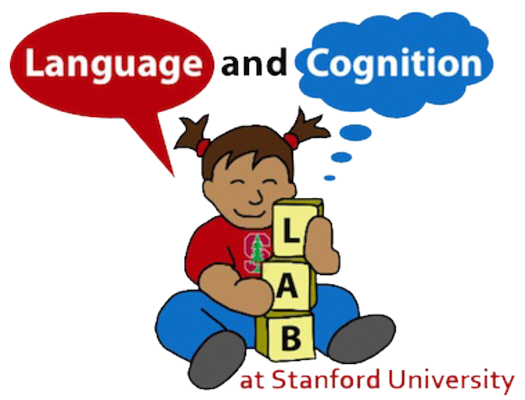
\includegraphics{figs/design_fig-1} 

}

\caption[Experimental design of behavioral task]{Experimental design of behavioral task: Adults watched sequences of stimuli consisting a familiarization to a stimulus (left), following by one of five trial types, which violates one property of the familiar stimulus: In the violation trials, participants saw either (1) the same exact stimulus (Background), (2) the same stimulus in a different orientation (Pose), (3) the same stimulus, but duplicated (or single if it was already duplicated; Number), (4) a different stimulus but in the same animacy class (Identity), or (5) a different stimulus of the opposite animacy (Animacy).}\label{fig:design_fig}
\end{figure}
\end{CodeChunk}

\hypertarget{methods}{%
\subsection{Methods}\label{methods}}

\hypertarget{stimuli}{%
\subsubsection{Stimuli}\label{stimuli}}

All stimuli were created using images selected from Unity assets Quirky
Series - Animals (LINK) and 3D Prop Vegetables and Fruits (LINK) with
added shaking animation. For each image from the animal set, we created
a mirrored version to create an image with a different pose. Since most
stimuli from the vegetable set are symmetrical, the images were slightly
tilted before the mirroring.

\hypertarget{procedure}{%
\subsubsection{Procedure}\label{procedure}}

The experiment was a web-based self-paced experiment that consisted of
two phases. In the first phase, participants saw 24 blocks that
consisted of either two, four, or six trials. On each trial, a schematic
screen would rise up to reveal a stimulus behind it. Participants
pressed the spacebar to go on to the next trial after a minimum viewing
time of 500 ms, triggering the schematic screen to drop and raise again
to reveal the next stimulus.

Each participant saw eight types of repeating stimuli. The eight types
of stimuli include all combinations of the three features that each
include two levels: animacy (e.g.~animate or inanimate), number
(singleton or pair), and pose (facing left or right).

8 blocks consisted of one stimulus being repeatedly presented throughout
the block (i.e.~background trials). The remaining 16 blocks included two
stimuli, including one that was repeatedly present and one that deviated
from the trial. The deviant trial was always different from the
repeating stimulus in one of the four dimensions: animacy violation,
identity violation, number violation, and pose violation. The deviant
trial always showed up in the last trial of the block. In the first
three violation types, the feature would be switched to the previously
unseen level (e.g.~an inanimate deviant after an animate repeating
stimulus, keeping the number and the pose the same). For identity
violation, the participants would see a different, but within-category,
exemplar from the repeating stimuli type. Among the sixteen blocks, the
four violation type each appeared four times. After each block,
participants performed a simple memory task as a filler task.

The order of the block was semi-randomized. To control for the
distribution of background blocks and deviant blocks, we group the
twenty-four blocks into four groups. Each group consisted of two
background blocks, and one deviant block from each violation type. The
order of blocks within each group was randomized.

\hypertarget{participants}{%
\subsubsection{Participants}\label{participants}}

The final sample included XXX participants recruited from Prolific(Mean
Age: SD:). Participants were excluded if either (1) the standard
deviation of log-transformed of their reaction times on all trials is
less than 0.15 (indicating key-smashing); (2) spent more than three
absolute deviations above the median of the task completion time as
reported by Prolific, or (3) provided the incorrect response to more
than 20\% of the memory task. After the participant-level exclusion, we
also applied trial-level exclusion. A trial was excluded from final
analysis if it is three absolute deviations away from the median in the
log-transformed space across all participants.

\hypertarget{results}{%
\subsection{Results}\label{results}}

The sample size and analysis plan are all pre-registered and can be
found here {[}LINK{]}. All experimental materials are publicly available
and can be found here {[}LINK{]}.

We were primarily interested in (1) whether our experimental paradigm
captured habituation and dishabituation and (2) whether the magnitude of
dishabituation was influenced by the type of violation. We tested these
two hypotheses in a linear mixed-effect model with maximal random effect
structure that predicts log-transformed looking time with the following
specification: log(total\_rt) \textasciitilde{} trial\_number +
is\_first\_trial + (trial\_number + is\_first\_trial) * number +
(trial\_number + is\_first\_trial) * pose +(trial\_number +
is\_first\_trial) * animacy + (trial\_number + is\_first\_trial) *
trial\_type. The combination of trial\_number and is\_first\_trial
models habituation.

interaction between trial number number and whether the trial is the
first trial models the habituation effect, testing the first hypothesis.
The following three interactions investigates whether the feature of
background trials would have an impact on the looking time. The last
interaction term, with trial type having five levels (background trial
or four types of violation), aims to test the second hypothesis. The
model with maximum random effect structure failed to converge, so we
pruned the model following the pre-registered procedure. The final model
included per-subject random intercepts.

There was also some evidence that participants showed graded
dishabituation to different types of violation. Animacy violation was
significantly greater than the number violation (STATS) as well as the
number violation (STATS). We also pre-registered a qualitative
prediction on the ordering of the dishabituation magnitude
(i.e.~category \textgreater{} number \textgreater{} identity
\textgreater{} pose). However, we did not find evidence consistent with
this prediction. The qualitative ordering in our data was animacy (M,
SD), identity (M, SD), pose (M, SD) and number (M, SD).

\hypertarget{model}{%
\section{Model}\label{model}}

We next wanted to ask whether looking time in our task can be seen as
rational information acquisition, using a ``rational analysis'' approach
previously described for a variety of aspects of human behavior
\cite{chater, dubey}. To do so, we developed RANCH, a Bayesian
perception/action model, in which a learner makes optimal perceptual
sampling decisions to maximize its learning
\cite{cao2023habituation, raz2023modeling}. To the extent that the model
behaves similarly to behavior observed in our task, we can argue that
human behavior on this task is optimized for perceptual learning.

Our goal was to develop a model which formalizes the entire process
underlying looking time: from perception of a stimulus to deciding how
long to look at it. To do so, our model has three separate components
describing 1) how RANCH takes raw images and embeds them into a
low-dimensional perceptual space, 2) how RANCH learns a concept over
this perceptual space and 3) how RANCH makes decisions about how long to
sample from a stimulus based on its expected information gain. Here, we
describe these three components in turn.

\begin{CodeChunk}
\begin{figure}[H]

{\centering 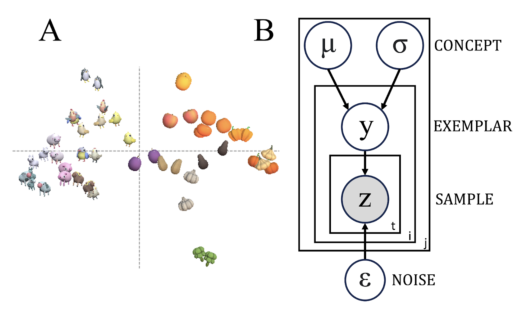
\includegraphics{figs/model_fig-1} 

}

\caption[A]{A: Stimulus embeddings in PC-space (showing first two components only for visualization purposes). (B) Plate diagram of the learning model, which learns distributions over a mean and standard deviation from noisy perceptual samples. t refers to the number of samples taken from y, i is the number of exemplars shown from the concept, and j is the number of features of the concept.}\label{fig:model_fig}
\end{figure}
\end{CodeChunk}

\hypertarget{perceptual-representation}{%
\subsection{Perceptual representation}\label{perceptual-representation}}

To allow RANCH to operate on raw images, we used perceptual embeddings
obtained from a model presented recently by Lee \& DiCarlo. This deep
neural network uses ResNet50 for encoding and then projects the final
layer onto a lower-dimensional embedding. This final projection is
``perceptually-aligned'', in that it was trained to match perceptual
dissimilarity matrices derived from human adult reaction times in a
2-AFC match-to-sample task. We use these projections into a
perceptually-aligned embedding space as a principled low-dimensional
representation of stimuli, over which our learning model can form
perceptual concepts. We used the first three principal components of the
embedding space. A visualization of experimental stimuli in the
embedding space can be seen in Figure 2A.

\hypertarget{learning-model}{%
\subsection{Learning model}\label{learning-model}}

RANCH's goal is to learn a concept in the perceptual embedding space
described above, through noisy perceptual samples from a stimulus. The
concept is parameterized by a 3D Gaussian \((\mu,\sigma)\), which
represents beliefs about the location and variance of the concept in the
embedding space. This concept \((\mu,\sigma)\) generates exemplars
\((y)\): exemplars of the concept. RANCH observes repeated noisy samples
\((\bar{z})\) from each exemplar. For any sample \((z)\) from an
exemplar \((y)\), the model expects the observation to get corrupted by
zero-mean noise, represented by \((\epsilon)\). A plate diagram is shown
in Figure 1B. We used a normal-inverse-gamma prior on the concept, the
conjugate prior for a normal with unknown mean and variance, on the
concept parameterized as \(\mu_{p}\),\(\nu_{p}\),\(\alpha_{p}\),
\(\beta_{p}\). Still, applying perceptual noise to \(y\) breaks the
conjugate relation, so we computed approximate posteriors using grid
approximation over \((\mu,\sigma)\) and \((\epsilon)\).

\hypertarget{decision-model}{%
\subsection{Decision model}\label{decision-model}}

To decide whether to take an additional sample from the same stimulus,
RANCH computes expected information gain (EIG) of the next sample. EIG
is computed as the product of the posterior predictive probability of
the next sample and the information gained conditioned on that next
sample, by iterating through a grid of possible subsequent samples.
RANCH then makes a softmax choice (with temperature = 1) between taking
another sample and looking away. We assumed that participants expect a
constant information gain from looking away (the ``world EIG'').
Therefore, as EIG from the stimulus drops below world EIG, it becomes
increasingly likely that RANCH will look away.

\hypertarget{simulating-the-experiment}{%
\subsection{Simulating the experiment}\label{simulating-the-experiment}}

To model the behavioral experiment, we first extracted the first three
principal components of the embeddings of all the stimuli used in the
experiment. We assembled the stimuli into sequences following the
stimuli sequence participants saw in each block. For the block with
deviating stimuli, we sampled deviant stimuli from corresponding
violation categories. We sampled 23 stimuli pairs for each combination
of violation type and deviant position. Since the model makes stochastic
sampling decisions, we conducted 400 runs for each stimuli sequence for
each parameter setting.

\hypertarget{alternative-models}{%
\subsection{Alternative models}\label{alternative-models}}

To test the importance of each of RANCH's components for its
performance, we defined three lesioned models. First, to test the
importance of the perceptual embeddings, we ran a version of RANCH in
which the mappings from stimulus labels to embeddings were permuted,
such that which embedding was associated with which violation type was
randomized (``Random embeddings''). Second, we ran a version in which
RANCH assumes that each perceptual sample in the learning process is
noiseless, rather than corrupted by \(\epsilon\) (``No noise'').Third,
we ran a version in which RANCH made decisions randomly rather than
based on the learning model (``No learning'').

\hypertarget{model-evaluation}{%
\section{Model Evaluation}\label{model-evaluation}}

\hypertarget{parameter-generalizability}{%
\subsubsection{Parameter
generalizability}\label{parameter-generalizability}}

RANCH was previously evaluated with behavioral data obtained from a
different task. In CITE, participants, both participants and models were
presented with a different set of stimuli. Unlike the current study, the
previous experiment only contained ``identity violation''.

We found that using these previously obtained parameters, RANCH
predicted the current task well (rsquared: RMSE: ). Qualitatively, it
shows the ordering of the graded dishabituation similar to the
behavioral data: animacy(M) \textgreater{} identity (M) \textgreater{}
pose (M) \textgreater{} number (M).

\hypertarget{parameter-robustness}{%
\subsubsection{Parameter robustness}\label{parameter-robustness}}

To evaluate RANCH's robustness to different parameters, we conducted a
grid search over the parameters. For each parameter setting, we
conducted a 10-fold cross-validation on the behavioral results.

Across the N parameter setting, the k-fold validation yields a moderate
range of R-squared (Mean; SD: )and RMSE (Mean: SD). When fit to the full
dataset, the fit of the winning parameter from this search was
comparable with the previous fit (rsquared; RMSE;). In addition, it also
preserved the qualitative ordering of the graded dishabituation
(Animacy: M; Identity (M)\ldots)

\hypertarget{comparison-with-alternative-models}{%
\subsubsection{Comparison with alternative
models}\label{comparison-with-alternative-models}}

Finally, to examine whether the assumptions in our models are critical
to the success of our models, we ran three alternative models: Random
Embedding model, No Noise model, and No Learning Model. We ran a
parameter search for each of the model, and all of the models showed
worse performance compared to RANCH (STATS).

\begin{CodeChunk}
\begin{figure*}[h]

{\centering 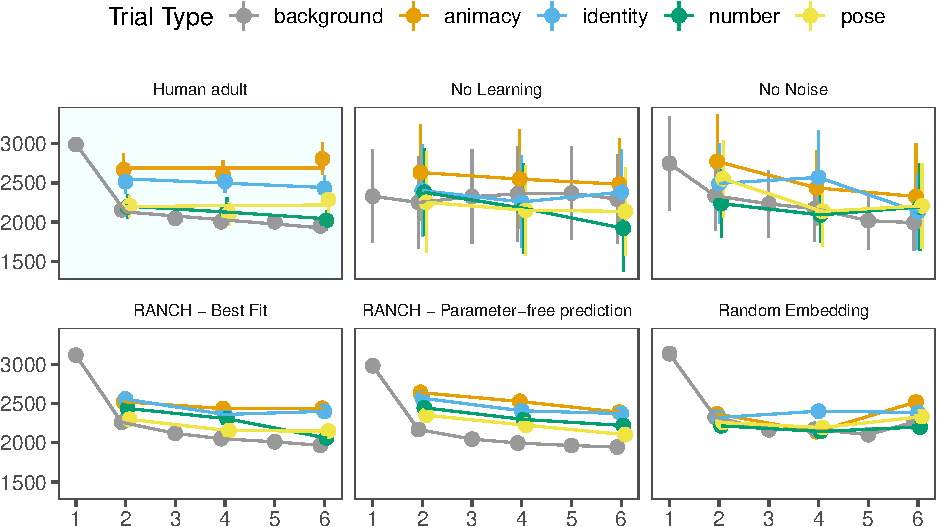
\includegraphics{figs/lol-1} 

}

\caption[This image spans both columns]{This image spans both columns. And the caption text is limited to 0.8 of the width of the document.}\label{fig:lol}
\end{figure*}
\end{CodeChunk}

\hypertarget{discussion}{%
\section{Discussion}\label{discussion}}

In this paper, we report on a novel experiment in which participants are
familiarized to sequences of animations, and we measure habituation and
their dishabituation to different types of violations of familiar
stimuli. We find that adults' dishabituation is graded by the type of
violation they see, and that the magnitude of dishabituation is
predicted by a rational model which takes noisy samples from perceptual
embeddings of the same stimuli that participants saw.

Our model, RANCH, through its use of perceptual embeddings, operates
directly on raw images and therefore can generate predictions for
previously unseen stimuli or even tasks. Making use of this property, we
tested RANCH's performance on our graded dishabituation task using
parameters fit to behavior on a completely different self-paced looking
timefree-viewing task \{raz2023modeling\} another behavioral task.

Lesioning RANCH by removing key components caused its performance to
drop significantly relative to its original implementation. This
suggests that the aspects that we lesioned - noisy perception,
connecting sampling to concept learning and a psychologically-plausible
embedding space - are essential for explaining behavior in our task.

Our work is limited in a variety of ways: First, in the current work, we
implemented a version of RANCH which takes a specific form for each of
its components: the perceptual representation, the learning model and
the linking hypothesis between learning and attentional sampling.
However, RANCH's modular and interpretable structure allows researchers
to adjust its components according to the population or task for which
predictions are being generated. For example, the perceptual embedding
space used in this paper was aligned to adult behavior @lee2022rapid,
but infants likely represent visual objects differently from adults.
Using perceptual representations based on visual input experienced by
infants may provide a better fit to infant data \{Zhuang et al. (2021),
Orhan \& Lake (2023)\}. Similarly, task settings in which there was
hierarchical structure to the stimuli sequences would call for more
complicated learning models. In previous work we have also explored the
effect of varying the linking hypothesis by replacing the rational, but
computationally expensive, expected information gain (EIG) with
easier-to-compute information-theoretic quantities such as surprisal or
KL-divergence (Cao et al. (2023), Raz, Cao, Saxe, \& Frank (2023)).

Second, while inspired by infant looking time research, our current work
only has adult participants. Beyond encoding stimuli differently from
infants, adults may conceptualize our task differently from infants, and
experience different task demands. In particular, infants are quite
sensitive to changes in the number of objects that are displayed (REFS),
but in the current study, adults dishabituated to number violations as
little as to pose violations, the sublest violation in our task.
Conducting this study in infants may reveal qualitative differences
between infant and adult dishabituation. Furthermore, given the
interpretability of the model parameters we fit to behavior, conducting
the same experiment with infants may lead to interpretable developmental
differences in the model parameters, such as priors on perceptual noise
and prior uncertainty about the mean and standard deviation of
perceptual concepts.

Overall, our work presents a rational model, RANCH, which describes how
humans decide how long to look at stimuli. Using a psychologically
motivated visual encoding model allows RANCH to operate on raw images,
and generate predictions for previously unseen stimuli or tasks. We
think that the generality and interpretability of our model framework
constitutes a significant step towards predictive modeling of adult, and
eventually infant, looking time, thereby putting the field on firmer
ground.

\hypertarget{references}{%
\section{References}\label{references}}

\setlength{\parindent}{-0.1in} 
\setlength{\leftskip}{0.125in}

\noindent

\hypertarget{refs}{}
\begin{CSLReferences}{1}{0}
\leavevmode\vadjust pre{\hypertarget{ref-anderson1991human}{}}%
Anderson, J. R. (1991). Is human cognition adaptive? \emph{Behavioral
and Brain Sciences}, \emph{14}(3), 471--485.

\leavevmode\vadjust pre{\hypertarget{ref-aslin2007s}{}}%
Aslin, R. N. (2007). What's in a look? \emph{Developmental Science},
\emph{10}(1), 48--53.

\leavevmode\vadjust pre{\hypertarget{ref-baillargeon1985object}{}}%
Baillargeon, R., Spelke, E. S., \& Wasserman, S. (1985). Object
permanence in five-month-old infants. \emph{Cognition}, \emph{20}(3),
191--208.

\leavevmode\vadjust pre{\hypertarget{ref-blumberg2023protracted}{}}%
Blumberg, M. S., \& Adolph, K. E. (2023). Protracted development of
motor cortex constrains rich interpretations of infant cognition.
\emph{Trends in Cognitive Sciences}.

\leavevmode\vadjust pre{\hypertarget{ref-cao2023habituation}{}}%
Cao, A., Raz, G., Saxe, R., \& Frank, M. C. (2023). Habituation reflects
optimal exploration over noisy perceptual samples. \emph{Topics in
Cognitive Science}, \emph{15}(2), 290--302.

\leavevmode\vadjust pre{\hypertarget{ref-doshi2023cortical}{}}%
Doshi, F. R., \& Konkle, T. (2023). Cortical topographic motifs emerge
in a self-organized map of object space. \emph{Science Advances},
\emph{9}(25), eade8187.

\leavevmode\vadjust pre{\hypertarget{ref-fantz1963pattern}{}}%
Fantz, R. L. (1963). Pattern vision in newborn infants. \emph{Science},
\emph{140}(3564), 296--297.

\leavevmode\vadjust pre{\hypertarget{ref-haith1980rules}{}}%
Haith, M. M. (1980). \emph{Rules that babies look by: The organization
of newborn visual activity}. Lawrence Erlbaum Associates.

\leavevmode\vadjust pre{\hypertarget{ref-haith1998put}{}}%
Haith, M. M. (1998). Who put the cog in infant cognition? Is rich
interpretation too costly? \emph{Infant Behavior and Development},
\emph{21}(2), 167--179.

\leavevmode\vadjust pre{\hypertarget{ref-hebart2020revealing}{}}%
Hebart, M. N., Zheng, C. Y., Pereira, F., \& Baker, C. I. (2020).
Revealing the multidimensional mental representations of natural objects
underlying human similarity judgements. \emph{Nature Human Behaviour},
\emph{4}(11), 1173--1185.

\leavevmode\vadjust pre{\hypertarget{ref-kidd2012goldilocks}{}}%
Kidd, C., Piantadosi, S. T., \& Aslin, R. N. (2012). The goldilocks
effect: Human infants allocate attention to visual sequences that are
neither too simple nor too complex. \emph{PloS One}, \emph{7}(5),
e36399.

\leavevmode\vadjust pre{\hypertarget{ref-lee2022rapid}{}}%
Lee, M. J. (2022). \emph{Rapid visual object learning in humans is
explainable by low-dimensional image representations} (PhD thesis).
Massachusetts Institute of Technology.

\leavevmode\vadjust pre{\hypertarget{ref-lieder2020resource}{}}%
Lieder, F., \& Griffiths, T. L. (2020). Resource-rational analysis:
Understanding human cognition as the optimal use of limited
computational resources. \emph{Behavioral and Brain Sciences},
\emph{43}, e1.

\leavevmode\vadjust pre{\hypertarget{ref-liu2017ten}{}}%
Liu, S., Ullman, T. D., Tenenbaum, J. B., \& Spelke, E. S. (2017).
Ten-month-old infants infer the value of goals from the costs of
actions. \emph{Science}, \emph{358}(6366), 1038--1041.

\leavevmode\vadjust pre{\hypertarget{ref-oaksford1994rational}{}}%
Oaksford, M., \& Chater, N. (1994). A rational analysis of the selection
task as optimal data selection. \emph{Psychological Review},
\emph{101}(4), 608.

\leavevmode\vadjust pre{\hypertarget{ref-orhan2023can}{}}%
Orhan, A. E., \& Lake, B. M. (2023). What can generic neural networks
learn from a child's visual experience? \emph{arXiv Preprint
arXiv:2305.15372}.

\leavevmode\vadjust pre{\hypertarget{ref-paulus2022should}{}}%
Paulus, M. (2022). Should infant psychology rely on the
violation-of-expectation method? Not anymore. \emph{Infant and Child
Development}, \emph{31}(1), e2306.

\leavevmode\vadjust pre{\hypertarget{ref-raz2023modeling}{}}%
Raz, G., Cao, A., Saxe, R., \& Frank, M. (2023). Modeling habituation in
infants and adults using rational curiosity over perceptual embeddings.
In \emph{Intrinsically-motivated and open-ended learning workshop@
NeurIPS2023}.

\leavevmode\vadjust pre{\hypertarget{ref-raz2020learning}{}}%
Raz, G., \& Saxe, R. (2020). Learning in infancy is active, endogenously
motivated, and depends on the prefrontal cortices. \emph{Annual Review
of Developmental Psychology}, \emph{2}, 247--268.

\leavevmode\vadjust pre{\hypertarget{ref-schrimpf2020integrative}{}}%
Schrimpf, M., Kubilius, J., Lee, M. J., Murty, N. A. R., Ajemian, R., \&
DiCarlo, J. J. (2020). Integrative benchmarking to advance neurally
mechanistic models of human intelligence. \emph{Neuron}, \emph{108}(3),
413--423.

\leavevmode\vadjust pre{\hypertarget{ref-teglas2011pure}{}}%
Téglás, E., Vul, E., Girotto, V., Gonzalez, M., Tenenbaum, J. B., \&
Bonatti, L. L. (2011). Pure reasoning in 12-month-old infants as
probabilistic inference. \emph{Science}, \emph{332}(6033), 1054--1059.

\leavevmode\vadjust pre{\hypertarget{ref-yamins2014performance}{}}%
Yamins, D. L., Hong, H., Cadieu, C. F., Solomon, E. A., Seibert, D., \&
DiCarlo, J. J. (2014). Performance-optimized hierarchical models predict
neural responses in higher visual cortex. \emph{Proceedings of the
National Academy of Sciences}, \emph{111}(23), 8619--8624.

\leavevmode\vadjust pre{\hypertarget{ref-zhuang2021unsupervised}{}}%
Zhuang, C., Yan, S., Nayebi, A., Schrimpf, M., Frank, M. C., DiCarlo, J.
J., \& Yamins, D. L. (2021). Unsupervised neural network models of the
ventral visual stream. \emph{Proceedings of the National Academy of
Sciences}, \emph{118}(3), e2014196118.

\end{CSLReferences}

\bibliographystyle{apacite}


\end{document}
